\section{Mapping from DPV to ODRL}
\label{sec:mapping}

The DPV-ODRL mapping described in this paper
is being developed as part of the W3C DPVCG's activities\footnote{
    \href{https://www.w3.org/groups/cg/dpvcg/}{DPVCG's} mission is to develop vocabularies
    that support the implementation of regulations,
    standards, and approaches relevant to privacy and data protection,
    and how these are addressed in technologies, including AI.},
with the support of the W3C ODRL CG\footnote{
    \url{https://www.w3.org/groups/cg/odrl/}},
and it is available at \url{https://dev.dpvcg.org/mappings/odrl},
with \texttt{dpv-odrl} as the suggested prefix.
Furthermore,
this mapping is represented in an RDF format,
as an ODRL profile,
following the best practices documented in the
ODRL V2.2 Profile Best Practices report~\cite{steidl_odrl_2023}. 
This ensures compatibility with existing ODRL implementations
and policy evaluation mechanisms.

\subsection{Methodology}
\label{sec:methodology}

The mapping between DPV and ODRL is implemented
using semantic alignment mechanisms,
primarily through relations from the SKOS vocabulary\footnote{
    \url{http://www.w3.org/2004/02/skos/core\#}},
RDF and RDFS\footnote{
    \url{http://www.w3.org/1999/02/22-rdf-syntax-ns\#} and
    \url{http://www.w3.org/2000/01/rdf-schema\#}}, and
OWL\footnote{
    \url{http://www.w3.org/2002/07/owl\#}}.
The following alignment strategies were considered:
\begin{itemize}
    \item \textbf{Instantiation}: A \texttt{dpv-odrl} class is instantiated as an ODRL class
    \item \textbf{Specialisation}: One concept is more specific than the other
    \item \textbf{Hierarchy}: A strict ontology subclass relationship
    \item \textbf{Equivalence}: Concepts represent the same meaning
    \item \textbf{Approximation}: Concepts are very similar but not strictly equivalent
    \item \textbf{Association}: Concepts are related but not hierarchically
    \item \textbf{Disjointness}: Mutually exclusive concepts
\end{itemize}
Table~\ref{tab:mapping} provides an overview of these strategies,
the semantic property used for the mapping,
and examples.

\begin{table}[ht]
    \centering
    \caption{Mapping types of DPV and ODRL Concepts}
    \label{tab:mapping}
    \begin{tabular}{lll}
        \toprule
        \textbf{Alignment} & \textbf{Mapping Relation} & \textbf{Example} \\
        \midrule
        Instantiation & \texttt{rdf:type} & \texttt{dpv-odrl:Entity rdf:type odrl:Party .} \\
        Specialisation & \texttt{skos:broader} & \texttt{dpv-odrl:Recipient skos:broader odrl:recipient .} \\
        Hierarchy & \texttt{rdfs:subClassOf} & \texttt{dpv-odrl:NDA rdfs:subClassOf odrl:Policy .} \\
        Equivalence & \texttt{skos:exactMatch} & \texttt{dpv-odrl:Agent skos:exactMatch dpv:Agent .} \\
        Approximation & \texttt{skos:closeMatch} & \texttt{dpv-odrl:Use skos:closeMatch odrl:use .} \\
        Association & \texttt{skos:related} & \texttt{dpv-odrl:Duration skos:related odrl:elapsedTime .} \\
        Disjointness & \texttt{owl:disjointWith} & \texttt{dpv-odrl:NDA owl:disjointWith (odrl:Offer, ...) .} \\
        \bottomrule
    \end{tabular}
\end{table}
% Disjointment: \texttt{$P_1 \cap P_i = \varnothing \quad \forall i \neq 1$}

\subsection{DPV-ODRL Profile}
\label{sec:profile}

Through the mapping described in the previous section,
DPV concepts can function within ODRL policies as:
\begin{inlinelist}
    \item parties,
    \item actions,
    \item assets,
    \item left operands,
    \item rules, and
    \item policy types
\end{inlinelist}.
Figure~\ref{fig:mapping}
provides an overview of this mapping where all DPV taxonomies
are mapped into one or more of the previously mentioned ODRL constructs.

\begin{figure}[ht]
    \centering
    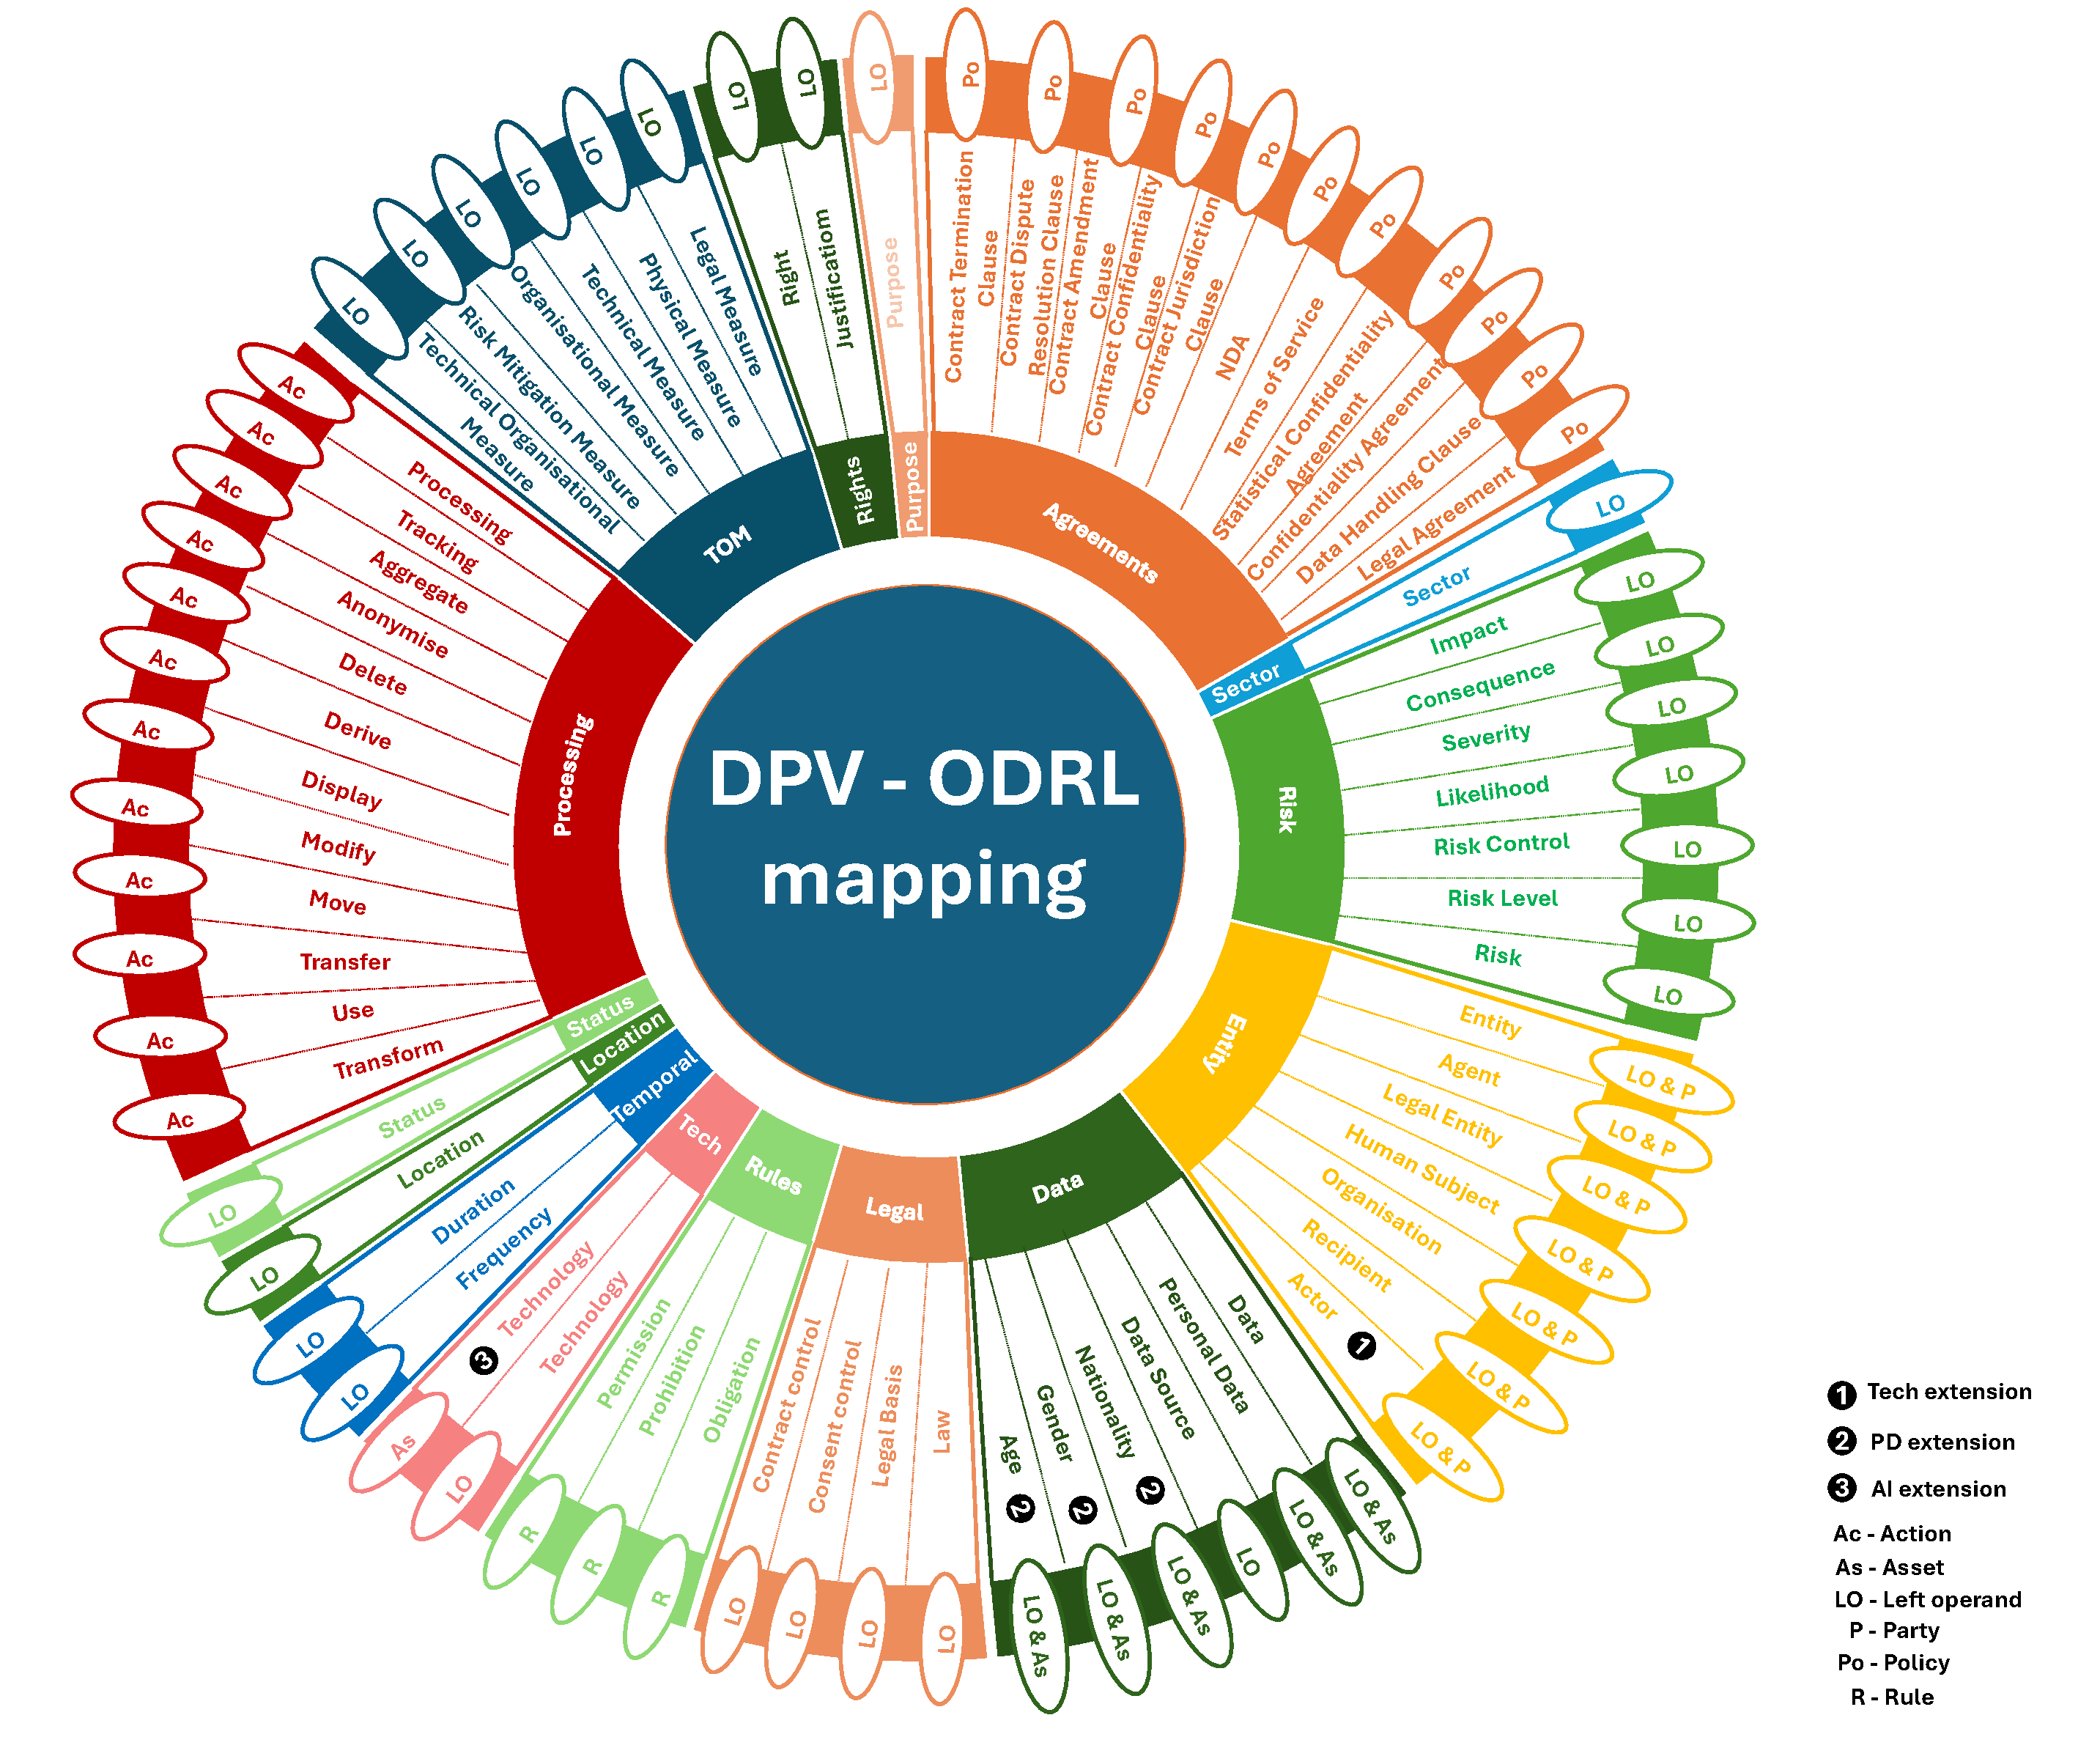
\includegraphics[width=\linewidth]{overview_cropped.pdf}
    \caption{Overview of DPV-ODRL mapping: the inner layer groups the terms by taxonomy, the middle layer contains the mapped DPV terms, and the outer layer contains the mapping to ODRL constructs.}
    \label{fig:mapping}
\end{figure}

\paragraph{Entities and Legal Roles}

DPV defines entities and legal roles
representing stakeholders involved in data processing activities,
such as individuals, organisations, institutions, or authorities.
As such,
they can be mapped as \texttt{odrl:Party} instances
and used as \texttt{odrl:assigner} or \texttt{odrl:assignee} of ODRL policies.
Furthermore,
due to the hierarchical structure of DPV,
certain entity concepts can be used as
left operands to filter ODRL party collections.
For example,
when a party collection contains multiple human subjects of different types,
the use of \texttt{dpv-odrl:HumanSubject} as the left operand
and \texttt{dpv:Patient} as the right operand
enables the specification of an ODRL policy
that applies exclusively to subjects of this particular type.
Listing~\ref{lst:entity} provides an example of a
DPV-ODRL mapping for entity concepts.
In this case,
\texttt{dpv-odrl:Recipient},
the equivalent to \texttt{dpv:Recipient},
is instantiated
as a \texttt{odrl:Party} and as a \texttt{odrl:LeftOperand},
and has a narrower scope than \texttt{odrl:recipient},
i.e., the right operand of \texttt{odrl:recipient}
is not restricted to a particular vocabulary,
while \texttt{dpv-odrl:Recipient} should require
a \texttt{dpv:Entity} as the right operand.

\begin{scriptsize}
\begin{lstlisting}[language=turtle, caption=DPV-ODRL mapping for the Recipient concept., label=lst:entity]
dpv-odrl:Recipient a odrl:Party, odrl:LeftOperand, skos:Concept ;
	skos:exactMatch dpv:Recipient ;
	skos:broader odrl:recipient .
    # add scope, e.g., which operators and right operand should be used
\end{lstlisting}
\end{scriptsize}

\paragraph{Processing Operations}

DPV processing concepts describe
operations that may be performed on data,
such as aggregation, deletion, transformation, or transfer.
These operations naturally correspond to ODRL actions and
can therefore be used to define
permitted, prohibited or mandatory activities within policies.
Furthermore, 
a few DPV processing terms closely correspond to existing ODRL actions,
allowing them to be related using the \texttt{skos:closeMatch}~---~%
Table~\ref{tab:processing} contains an overview of these terms.
Listing~\ref{lst:action} provides an example of a
DPV-ODRL mapping for a processing operation.
In this case,
\texttt{dpv-odrl:Use},
the equivalent to \texttt{dpv:Use},
is instantiated as an \texttt{odrl:Action} and
has a similar ODRL concept, i.e., \texttt{odrl:use}.

\begin{scriptsize}
\begin{lstlisting}[language=turtle, caption=DPV-ODRL mapping for the Use concept., label=lst:action]
dpv-odrl:Use a odrl:Action, skos:Concept ;
	skos:exactMatch dpv:Use ;
	skos:closeMatch odrl:use .
\end{lstlisting}
\end{scriptsize}

\begin{table}[ht]
    \centering
    \caption{Mapping of DPV processing operations to ODRL actions.}
    \label{tab:processing}
    \begin{tabular}{lll}
        \toprule
        \textbf{ODRL Concept} & \textbf{DPV Concept} & \textbf{Mapping Type} \\
        \midrule
        odrl:acceptTracking & dpv:Tracking & skos:closeMatch \\
        odrl:aggregate & dpv:Aggregate & skos:closeMatch \\
        odrl:anonymize & dpv:Anonymise & skos:closeMatch \\
        odrl:delete & dpv:Delete & skos:closeMatch \\
        odrl:derive & dpv:Derive & skos:closeMatch \\
        odrl:display & dpv:Display & skos:closeMatch \\
        odrl:modify & dpv:Modify & skos:closeMatch \\
        odrl:move & dpv:Move & skos:closeMatch \\
        odrl:transfer & dpv:Transfer & skos:closeMatch \\
        odrl:transform & dpv:Transform & skos:closeMatch \\
        odrl:use & dpv:Use & skos:closeMatch \\
        \bottomrule
    \end{tabular}
\end{table}

\paragraph{Data and Technologies}

In ODRL,
assets represent the resources targeted by policies.
On the other hand,
DPV provides a comprehensive taxonomy for describing data,
including categories of personal and non-personal data,
as well as a Personal Data Categories extension\footnote{
    \url{https://w3id.org/dpv/pd}},
which provides additional concepts to represent different types of personal data,
e.g., social, demographic, financial, or health-related data categories.
These concepts can therefore be mapped to ODRL assets,
but can also be used as left operands to refine asset or party collections
to specific demographic groups, e.g.,
to restrict the usage of a certain asset to parties which are over 18.
% TODO: include example in the next section that can be referenced here
Furthermore,
DPV provides technology-related concepts
that can be used to denote the use of any technological resources,
including AI systems.
These concepts can also be used as assets within ODRL policies
to specify conditions governing the use of such resources.
Furthermore, DPV's Technology\footnote{
    \url{https://w3id.org/dpv/tech}}
and AI Technology\footnote{
    \url{https://w3id.org/dpv/ai}}
extensions introduce additional technological concepts
that can be employed as assets or as further constraints in ODRL policies.
For example,
a policy may specify that a given asset may only be used for training an AI model.

\paragraph{Contextual and Governance-related Constraints}

The majority of DPV taxonomies yet to be discussed in this section
are mapped as ODRL left operands to further constrain ODRL policies.
The following list provides an overview of these taxonomies and
their utility to restrict ODRL policies:
\begin{itemize}
    \item \textbf{Purpose:} Purpose limitation is a central principle in many data protection frameworks, particularly the GDPR. DPV includes an extensive taxonomy of purposes, which can be integrated into ODRL policies to constrain data or technology usage to a particular purpose or set of purposes. This alignment enables the expression of policies such as allowing the use of a dataset exclusively for research or restricting its use to statistical analysis.
    \item \textbf{Technical and Organisational Measures:} Data protection regulations frequently require the implementation of safeguards such as encryption, authentication mechanisms, or organisational controls. DPV models such safeguards as technical and organisational measures (TOMs), which can be used as constraints within ODRL policies for, e.g., permitting access to a dataset only when multi-factor authentication is implemented.
    \item \textbf{Legal and Jurisdictional Constraints:} DPV location concepts can restrict asset usage to specific locations or jurisdictions, supported by the Location\footnote{\url{https://w3id.org/dpv/loc}} extension that contains concepts to represent countries and regions based on ISO 3166. Additionally, DPV provides concepts for representing applicable laws and legal bases for processing activities, with the Legal\footnote{\url{https://w3id.org/dpv/legal}} extensions supporting the modelling of laws and authorities across jurisdictions.
    \item \textbf{Time-based Context:} Temporal aspects of policies, including duration and frequency of usage, can also be represented through DPV concepts. These mappings allow policies to define how long data may be used or how often certain operations may occur. Furthermore, these DPV concepts can be related to a few ODRL left operands in a non-hierarchical way, e.g., \texttt{dpv:Duration} is related to \texttt{odrl:elapsedTime}. Listing~\ref{lst:duration} provides the DPV-ODRL mapping for duration, where \texttt{dpv-odrl:Duration}, the equivalent to \texttt{dpv:Duration}, is instantiated as an \texttt{odrl:LeftOperand} and has related ODRL concepts, i.e., \texttt{odrl:elapsedTime} and \texttt{odrl:count}.
    \item \textbf{Rights and Risks:} DPV includes concepts representing risks, rights, and justifications associated with processing activities. They can be used to justify the exercising of a certain right, e.g., a data subject wants to exercise their right to erasure given that the processing of their personal data is no longer required, or to restrict the use of assets when risk levels exceed certain thresholds.
    \item \textbf{Sector and Status:} DPV sector concepts can be used to permit or restrict asset usage based on the application domain. The AI Act\footnote{\url{https://w3id.org/dpv/legal/eu/aiact}} extension provides sector-related concepts, such as education and employment, to represent these domains. Additionally, DPV status concepts can indicate the state of processes or activities, enabling policies to constrain asset usage based on conditions such as the status of given consent.
\end{itemize}
A detailed list of these mappings
is available at \url{https://dev.dpvcg.org/mappings/odrl}
and can be observed in Figure~\ref{fig:mapping}.

\begin{scriptsize}
\begin{lstlisting}[language=turtle, caption=DPV-ODRL mapping for the Duration concept.,  label=lst:duration]
dpv-odrl:Duration a odrl:LeftOperand, skos:Concept ;
    skos:exactMatch dpv:Duration ;
	skos:related odrl:elapsedTime, odrl:count .
\end{lstlisting}
\end{scriptsize}

\paragraph{Rules}

\begin{scriptsize}
\begin{lstlisting}[language=turtle, caption=Secondary use policy for purposes associated with healthcare scientific research.,  label=lst:rule]
dpv-odrl:Obligation skos:exactMatch dpv:Obligation ;
	skos:closeMatch odrl:Duty .
\end{lstlisting}
\end{scriptsize}

\paragraph{Agreements}

\begin{scriptsize}
\begin{lstlisting}[language=turtle, caption=Secondary use policy for purposes associated with healthcare scientific research.,  label=lst:policy]
dpv-odrl:NDA a rdfs:Class, skos:Concept ;
    skos:exactMatch dpv:NDA ;
	rdfs:subClassOf odrl:Policy ;
	owl:disjointWith odrl:Agreement, odrl:Offer, odrl:Privacy, odrl:Request, odrl:Ticket, odrl:Assertion,
	dpv-odrl:ContractConfidentialityClause, dpv-odrl:ContractDisputeResolutionClause,
	dpv-odrl:ContractJurisdictionClause, dpv-odrl:ContractTerminationClause,
	dpv-odrl:TermsOfService, dpv-odrl:DataHandlingClause, dpv-odrl:LegalAgreement,
	dpv-odrl:ConfidentialityAgreement, dpv-odrl:NDA, dpv-odrl:StatisticalConfidentialityAgreement .
\end{lstlisting}
\end{scriptsize}